\documentclass{article}
\usepackage{xeCJK}
\usepackage{geometry}
\usepackage{amsmath}
\usepackage{graphicx}
\usepackage{listings}
\usepackage{xcolor}

\graphicspath{{./images/}}
\geometry{a4paper,scale=0.8}

\title{题目解答: 中国私募量化面试Q&A系列——白鹭资管}
\author{张西通}
\date{}
\begin{document}

\section{问题 1}
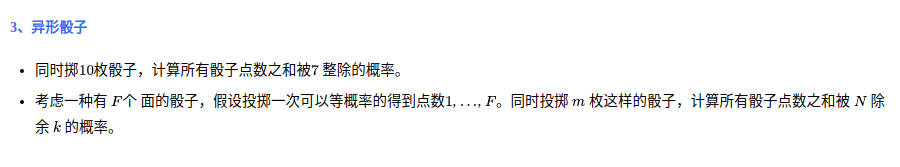
\includegraphics[scale=0.5]{dice.png}

1. 考虑一般情况,$P_n(x)$ 为投掷 n 个色子,和除以 7 余数为 x 的概率,则
$$
P_{n+1}(0) = \frac{1}{6} \times P_n(1) + \frac{1}{6} \times P_n(2) + ... + \frac{1}{6} \times P_n(6) = \frac{1}{6} \times (1 - P_n(0)) 
$$
由此可求得 $P_n(0)$ 的通项公式为
$$
P_n(0) = \frac{1}{7} - \frac{1}{7}\times(-\frac{1}{6})^{(n-1)}
$$
所以题目要求的 $P_{10}(0) = \frac{6^9 + 1}{7 \times 6^9} \approx \frac{6^9}{7 \times 6^9} = \frac{1}{7}$

\vspace{60pt}
2. 投掷m次的生成函数为
$$
g(x) = (x + x^2 + ... + x^F)^m = [\frac{x(1-x^F)}{1-x}]^m
$$

和 S 的取值范围为 $m <= S <= F \times m $。其中 除以 N 余数为 k 的数为 $ \alpha N + k $, $\alpha$ 为自然数。所以有
$$
\frac{m-k}{N} <= \alpha <= \frac{Fm-k}{N}
$$

余数为 k 的总的情况数有
$$
B = \Sigma_S g^{(S)} \times \frac{1}{S!} |_{x=0},  \alpha \in [\frac{m-k}{N}, \frac{Fm-k}{N}] 
$$

其中 $g^{(S)}$ 为 g 函数的 S 阶导数。

那么概率为
$$
P = \frac{B}{F^m}
$$





\newpage
\section{问题 2}
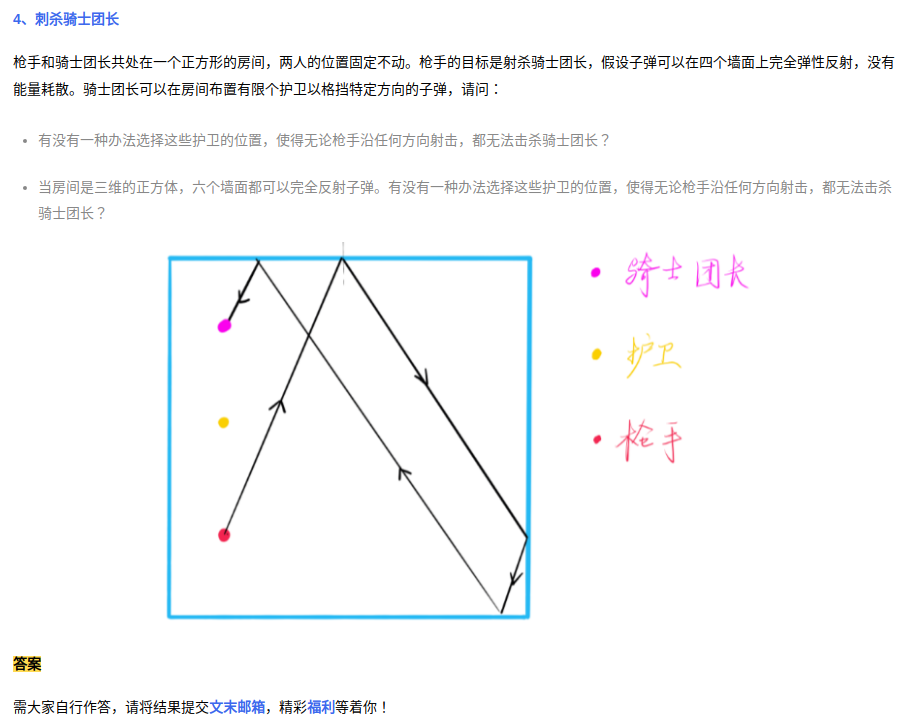
\includegraphics[scale=0.5]{knight.png}

我可能没有理解这个题目的玄机。我得到的结论是无法用有限个护卫来保护团长。

可以参考光的反射,正方形四条边都是镜子。如图,用圆点代表狙击手,用星星代表团长。可以画出狙击手所有镜面对称点,图中的虚线方格中的点。由于镜面互相反射,可以形成无穷多个枪手的镜像。从每个枪手的镜像点到团长连一条线,这条线就是一条可能的击杀团长的方向。而一个守卫只能保卫一个方向,而方向有无穷多个,所以无法用有限的守卫来保护团长。

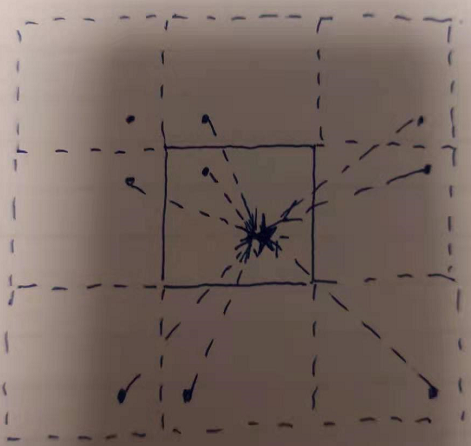
\includegraphics[scale=0.5]{mirror.png}



\newpage
\section{问题 3}
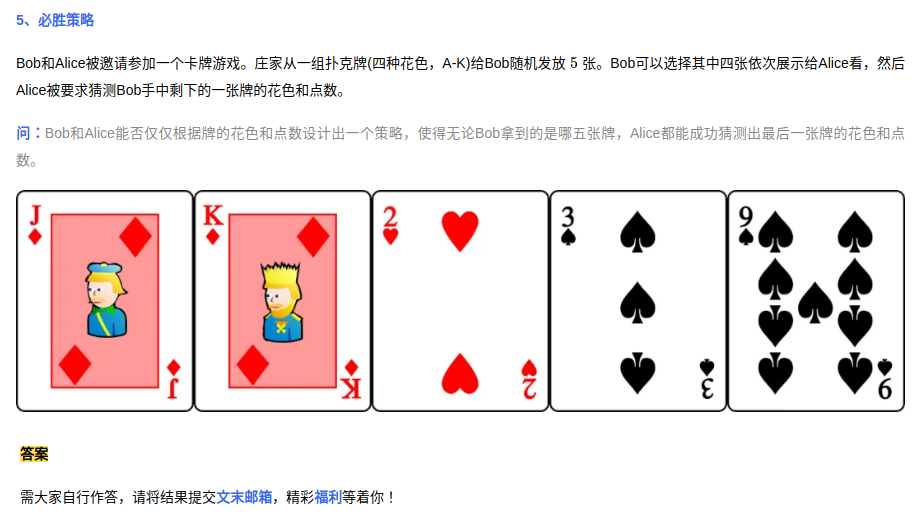
\includegraphics[scale=0.5]{puke.png}

(1) 开始之前,Bob 和 Alice 给每张牌从1-52编号,这样每张牌都有大小差别了。

(2)因为一共四种花色,必然至少有两张牌花色一样,Bob从这两张花色一样的牌里选一张作为Alice猜的牌,而另一张作为第一张出的牌。Bob根据第一张牌,就知道要猜测的牌的花色是什么。至于Bob从这两个里选哪张牌,后面讨论

(3)剩下的3张牌,不妨设他们的编号为1,2,3,那么就有3!种排列方式,可以编号1-6 六个数字。而此时Alice 已经知道了最后一张牌的花色,但不知道数字。数字有12种可能性。

(4)我们把1,2,3,4,… 12,13 顺时针放到一个圆盘上,会发现两个数距离最大是6,而这正是剩下三张牌可以表示的范围。所以,Bob在出第一张牌的时候,选择距离短的一段圆弧并且顺时针靠后的一张牌,然后用剩下三张牌的排序代表最后一个牌与第一个牌的差值。Alice只要根据第一张牌的数字,加上三张牌排序的数字,就得到最后一张牌的数字了。

(5)举例:题目中的例子,令2<J<K, Bob 第一次出 黑桃3,Alice知道了这个牌的花色是黑桃。然后 Bob 依次出 K, J, 2, 这个顺序在所有排序中位列第6个,所以表示数字6. Alice 此时用3 + 6 = 9 就知道最后一张牌的数字了。



\newpage
\section{问题 4}
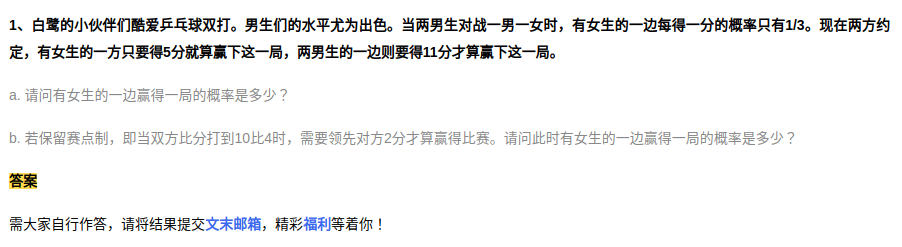
\includegraphics[scale=0.5]{pingpang.png}

a. 考虑女生输的情况的比分有 11:0, 11:1, 11:2, 11:3, 11:4,并且最有一分一定是男生得分。考虑一般情况 11:a的概率为
$$
P(a) = C^a_{10+a} \times (\frac{1}{3})^a \times (\frac{2}{3})^{11}
$$
所以女生输的总概率为
$$
P = \Sigma_{a=1}^{4} P(a) = [C^0_{10} + C^1_{11} \times (\frac{1}{3})^1 + C^2_{12} \times (\frac{1}{3})^2 + C^3_{13} \times (\frac{1}{3})^3 + C^4_{14} \times (\frac{1}{3})^4] \times (\frac{2}{3})^{11} = 0.4040647834709638
$$

所以女生赢一局的概率为 $ 1 - P = 0.5959352165290361 $

\vspace{60pt}

b. 若保留赛点制,前面的计算中,除了11:4的情况外,其他都适合。下面求11:4的情况。
比分为10:4的概率为
$$
P_0 = C^4_{14} \times (\frac{1}{3})^4 \times (\frac{2}{3})^{10}
$$

那么接下来女生要输,可能还要打2个球,4个球,6个球...,并且最后两个球一定是男生连续赢2个。考虑一般情况,再打 a 个球女生输了,a为偶数,那么概率为
$$
P(a) = P_0 \times (\frac{1}{3} \times \frac{2}{3} + \frac{2}{3} \times \frac{1}{3})^{\frac{a-2}{2}} \times (\frac{2}{3})^2 = P_0 \times (\frac{4}{9})^b
$$
其中 $b=\frac{a}{2} = 1,2,3,...$

那么,赛点后女生输的概率为
$$
P_1 = \Sigma^{\infty}_{b=1} P(a) = \Sigma^{\infty}_{b=1}(\frac{4}{9})^b \times P_0 = \frac{4}{5} \times P_0 = 0.17144564390862652
$$

那么女生输的概率为
$$
P = [C^0_{10} + C^1_{11} \times (\frac{1}{3})^1 + C^2_{12} \times (\frac{1}{3})^2 + C^3_{13} \times (\frac{1}{3})^3] \times (\frac{2}{3})^{11} + P_1 = 0.43263905745573483
$$

所以女生赢的概率为 $ 1 - P = 0.5673609425442652 $

\newpage

\section{问题 5}

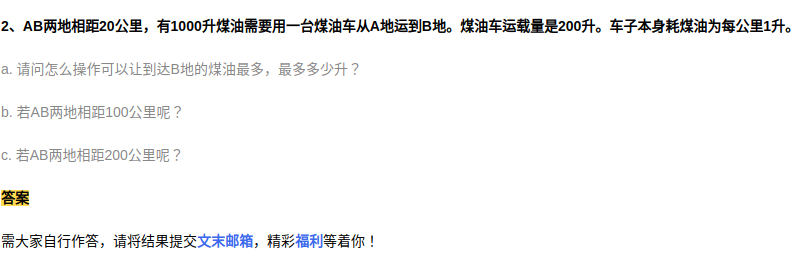
\includegraphics[scale=0.5]{oil.png}

此题就是让车能够移动最少的距离然后把油从A运送到B。考虑AB距离为L,他们的中点为C,如果我们先把油从A运到C,再从C运到B,在这种方案下,A到C的来回次数和原来A到B的来回次数相同。由于在C点的油已经小于在A点的油,所以C到B的来回次数可能要小于原来A到B的来回次数。所以先把所有油运到中点,一定是优于直接从起始点运到末尾。因此,我们把AB这段距离分割的次数越多,油耗就会越小。
设当所有油运到了$x$处,此时总油量为$a$,那么我们运到下一个$x+dx$处,油量变化为$da$
令 
$$ a = 200k+ b $$
即 $ b = a \% 200 $, $k$ 为整数。
则油罐车在这段$ dx $ 上的往返次数为(因为$dx$可以取无限小,所以只要$b > 0$,总可以使得 $b > 2dx$ 成立, 油罐车总要回去把剩余的$b$取来)
$$ 
n = \left\{
    \begin{aligned}
        2k - 1 & , & b = 0 \\
        2k + 1 & , & b > 0 
    \end{aligned}
\right.
$$
所以往前运输 $dx$ 这段距离上的油耗为 $n \times dx$ 所以可以得到每公里油耗$C(a)$为:
$$
C(a) = \frac{da}{dx} = n = 
\left\{
    \begin{aligned}
        9 & , & a \in [1000, 800) \\
        7 & , & a \in [800, 600) \\ 
        5 & , & a \in [600, 400) \\
        3 & , & a \in [400, 200) \\
        1 & , & a \in [200, 0) \\
    \end{aligned}
\right.
$$

所以可以求得问题中的解:


当 AB 距离 20km 时候,油耗 = 9L/km, 所以到达 B 处时候最大油量为 $1000 - 9 \times 20 = 820$

当 AB 距离为 100km 时候, 到达B 处的最大油量为
$$ 
400 - (100 - (\frac{200}{9} + \frac{200}{7} + \frac{200}{5})) \times 3 = 372.3809523809524
$$


当 AB 距离为 200km的时候,到达B 处的最大油量为
$$
200 - (200 - (\frac{200}{9} + \frac{200}{7} + \frac{200}{5} + \frac{200}{3})) \times 1 = 157.46031746031747
$$

\newpage
\section{问题6}
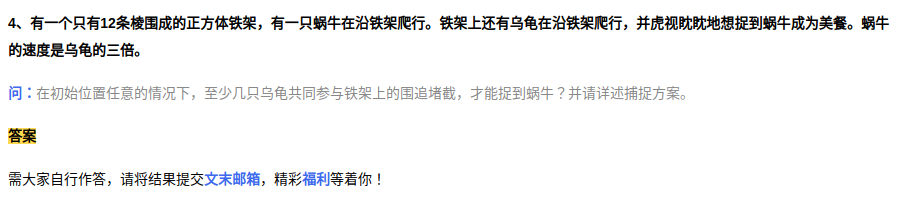
\includegraphics[scale=0.5]{turtle.png}

最少需要 3 只乌龟。首先 1 只乌龟显然追不上。2 只乌龟时候,只要蜗牛一直保持不跟那两只乌龟在同一个面上就不会被抓到。下面给出 3 只乌龟一定能抓到的策略:

3 只乌龟先不管蜗牛的位置,直接走到图中 A, B, C 三个点。此时,蜗牛有三种情况:(1)在D点、(2)在E点(于F、G两点等效), (3)在DE中间

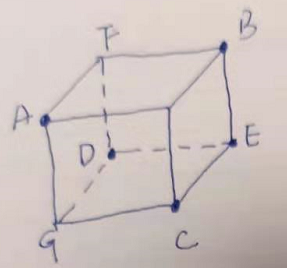
\includegraphics[scale=0.5]{cube01.png}

\vspace{60pt}

现在分别讨论这三种情况

情况1: 乌龟在A、B、C三点,蜗牛在D点。此时,三只乌龟运动方向如图箭头所示。当三只乌龟分别走了$\frac{1}{3}$ 棱长的时候,此时如果蜗牛运动到了E点(其他两点等效),那么B乌龟要观察蜗牛的下一步运动,如果蜗牛要往B点走,那么B乌龟就要掉头返回也往B走。因为蜗牛速度是乌龟3倍,所以蜗牛最快也只能和B乌龟相遇在B点被捕捉。如果蜗牛不往B走了,B蜗牛就继续望F走。否则就继续往前走。按照这个策略一直走,三只乌龟最终会在G、F、E点,而蜗牛就被困在了D、E之间。最终会被抓到。

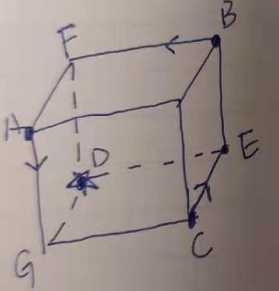
\includegraphics[scale=0.5]{cube02.png}

\vspace{60pt}

情况2: 乌龟在A、B、C三点,蜗牛在E点。A 乌龟想G点移动,而B、C乌龟观察E点处蜗牛的运动。若蜗牛从E点往D点走,则B蜗牛往F走,C蜗牛网E走。这样走下去,最终会到情况1中的状态而被捕获。若E处蜗牛中途返回E,则B、C乌龟也分别返回。当A蜗牛到达G点时候,若蜗牛在E点,则其他两只乌龟在B、C点,此时乌龟观察E点的蜗牛的运动,若E不动,则G点乌龟往D走,若E向D走,则B->F,C->E,G点乌龟不动。这样最终也会达到情况1中的 状态而被捕获。

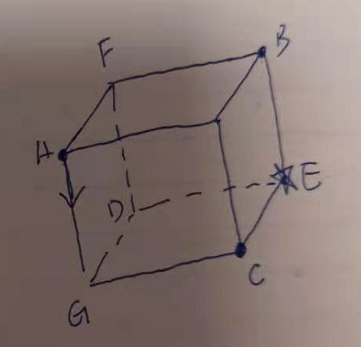
\includegraphics[scale=0.5]{cube03.png}

\vspace{60pt}

情况3: 乌龟在A、B、C三点,蜗牛在D、E中间。前面两种情况,蜗牛在D点和E点都必然被捕获,在中间最后总会落到情况1、2中的一种。所以必然也会被捕获。

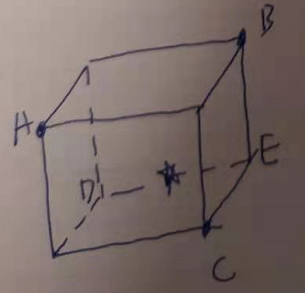
\includegraphics[scale=0.5]{cube04.png}

由此,最少需要 3 只乌龟就可以捉住蜗牛。



\newpage
\section{问题 7}
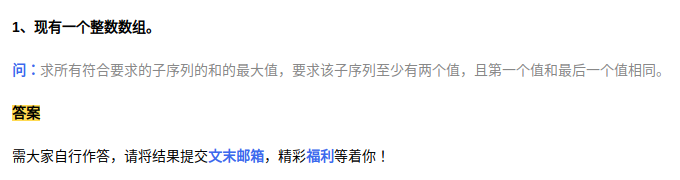
\includegraphics[scale=0.7]{algo.png}

因为我是做IT的,做的算法题比较多。对于这个题目,有两点可以改进。第一,算法题要给出数据范围。比如这个数组多大?数组中每个数多大?因为数据范围直接决定了需要采取的算法。第二,需要说明子序列的定义。在计算机算法这边,子序列是指给定一个序列,删掉任意个元素后得到的序列。我就按照这个定义来做这个题目。

思路: 用一个idxs来记录每个数字出现的坐标。只需要知道每个数第一个index和最后一个index。另外记录一个数组 sps, sps[i] 的含义是从 0到i之间(包含0,i),所有nums中非负数的和,这个数组主要是可以用O(1)的复杂度来获得任意区间内非负数的和。准备好这两个后,遍历 idxs中的数 a ,如果这个数 a 出现次数>=2,那么就取第一个和最后一个的index,分别为b,e,然后求得b到e之间(不包含b,e)的所有非负数的和,加上2*a 就是以a为头尾的最大的子序列的和,记为cur。然后在所有cur中找到一个最大的就好了。

时间复杂度:O(n)

代码:

\lstset{
 columns=fixed,       
 numbers=left,                                        % 在左侧显示行号
 numberstyle=\tiny\color{gray},                       % 设定行号格式
 frame=none,                                          % 不显示背景边框
 backgroundcolor=\color[RGB]{245,245,244},            % 设定背景颜色
 keywordstyle=\color[RGB]{40,40,255},                 % 设定关键字颜色
 numberstyle=\footnotesize\color{darkgray},           
 commentstyle=\it\color[RGB]{0,96,96},                % 设置代码注释的格式
 stringstyle=\rmfamily\slshape\color[RGB]{128,0,0},   % 设置字符串格式
 showstringspaces=false,                              % 不显示字符串中的空格
 language=python,                                        % 设置语言
}
\begin{lstlisting}
def maxSum(nums: list)->int:
    n = len(nums)
    sps = [0] * n
    idxs = {}
    for i in range(n):
        a = nums[i]
        if a not in idxs:
            idxs[a] = []
        idxs[a].append(i)

        if a >= 0:
            sps[i] = a
        if i > 0:
            sps[i] += sps[i-1]

    def querySum(b:int, e:int):
        if b > e:
            return 0
        res = sps[e]
        if b > 0:
            res -= sps[b-1]
        return res

    res = None
    for a in idxs:
        if len(idxs[a]) > 1:
            b, e = idxs[a][0], idxs[a][-1]
            cur = querySum(b+1, e-1) + 2*a

            if res is None or cur > res:
                res = cur
    return res

if __name__ == '__main__':
    # case1: all negative
    print(maxSum([-1,-2,-1]))
    # case2: no same item
    print(maxSum([1,2,3]))
    # case3: all positive
    print(maxSum([1,2,1,2]))
    # case4: 
    print(maxSum([1,-1,-1,1]))

\end{lstlisting}

\end{document}